\chapter{Étude de deux oscillateurs de Van der Pol couplés}
%
Étudions maintenant le système suivant, composé de deux oscillateurs de Van der Pol identiques, couplé par une force de rappel linéaire relativement faible. On cherchera à étudier si les oscillateurs se synchronisent, et la manière dont ils se synchronisent.
%
\begin{equation}
  \left\{\begin{array}{@{}l@{}}
    \ddot{x}_1 + x_1  + \epsilon(x_1^2 - 1)\dot{x}_1 = \epsilon k(x_2 - x_1) \\
    \\
    \ddot{x}_2 + x_2 + \epsilon(x_2^2 - 1)\dot{x}_2 = \epsilon k(x_1 - x_2)
  \end{array}\right.\,
  \label{eq:coupled_vdp}
\end{equation}
%
Encore une fois, on procède par la méthode de moyennement pour obtenir une approximation de l'enveloppe lentement variable :
%
\begin{equation}
    2\dot{z}_1(t) = 
     \epsilon \left[ z_1(t) - |z_1|^2z_1(t) \right]
    - i\epsilon k\left( z_2(t) - z_1(t)\right)
\end{equation}
%
On sépare les parties réelles des parties imaginaires et on obtient un système d'équation pour $\dot{r}_1$,  $\dot{r}_2$,  $\dot{\phi}_1$ et  $\dot{\phi}_2$. %le système :
%
%
%   \begin{equation}
%       \left\{\begin{array}{@{}l@{}}
%         \dot{r}_1 = \frac{\epsilon}{8} r_1 \left( 4 - r_2^2 \right) + k\frac{r_2}{2}\sin(\phi_2 - \phi_1)\\
%         \\
%         \dot{r}_2 = \frac{\epsilon}{8} r_2 \left( 4 - r_2^2 \right) + k\frac{r_1}{2}\sin(\phi_1 - \phi_2)\\
%         \\
%         \dot{\phi}_1 = \frac{k}{2}\left( 1 - \frac{r_2}{r_2}\cos(\phi_2 - \phi_1)\right) \\
%         \\
%         \dot{\phi}_2 = \frac{k}{2}\left( 1 - \frac{r_1}{r_2}\cos(\phi_1 - \phi_2)\right)
%       \end{array}\right.\,
%    \end{equation}
%
%
Or, l'oscillateur de Van der Pol n'ayant pas de phase de référence (sa phase n'étant pas fixée par une force extérieure), 
%la phase des deux oscillateurs peuvent se synchroniser. En effet, 
l'évolution du système ne dépend que de la différence entre les phases des oscillateurs. 
On peut donc réduire le système à trois équations en introduisant la variable de déphasage $\Theta = \phi_2 - \phi_1$ :
%
\begin{equation}
    \left\{\begin{array}{@{}l@{}}
        \dot{r}_1 =  \frac{\epsilon}{8} r_1 \left( 4 - r_2^2 \right) + \epsilon k\frac{r_2}{2}\sin(\phi_2 - \phi_1)\\
        \\
        \dot{r}_2 =  \frac{\epsilon}{8} r_2 \left( 4 - r_2^2 \right) + \epsilon k\frac{r_1}{2}\sin(\phi_1 - \phi_2)\\
        \\
        \dot{\phi}_1 = \epsilon \frac{k}{2}\left( 1 - \frac{r_2}{r_1}\cos(\phi_2 - \phi_1)\right) \\
        \\
        \dot{\phi}_2 = \epsilon \frac{k}{2}\left( 1 - \frac{r_1}{r_2}\cos(\phi_1 - \phi_2)\right)
    \end{array}\right.\,
    \implies
    \left\{\begin{array}{@{}l@{}}
        \dot{r}_1 = \frac{\epsilon}{8} r_1 \left( 4 - r_2^2 \right) + \epsilon k\frac{r_2}{2}\sin(\Theta)\\
        \\
        \dot{r}_2 = \frac{\epsilon}{8} r_2 \left( 4 - r_2^2 \right) - \epsilon k\frac{r_1}{2}\sin(\Theta) \\
        \\
      \dot{\Theta} = \epsilon \frac{k}{2}\left(  \frac{r_2}{r_1} - \frac{r_1}{r_2} \right)\cos(\Theta)
    \end{array}\right.\,
  \end{equation}
  %
  On s'intéresse aux solutions stationnaires. Pour cela, on s'inspire du cas non couplé. Lorsque $k=0$, la configuration stable correspond à $r_1 = r_2 = 2 $
avec $\Theta$ arbitraire.
%
On cherche s'il y a quelque chose de similaire pour $k \neq 0$. Si on pose :
\[r_1 = r_2 = 2 \quad \text{et} \quad \dot{r}_1 = \dot{r}_2 = \dot{\Theta} = 0\]
On trouve effectivement une solution stationnaire à condition que $\Theta = 0$ ou $\Theta = \pi$. Donc il existe au moins deux solutions stationnaires, une où les deux oscillateurs sont en phase, et une autre en anti-phase.
%
\section{Analyse de stabilité linéaire}
%
Pour déterminer la stabilité de ces solutions stationnaires, on peut faire une analyse de stabilité linéaire dans le voisinage des solutions stationnaires. On notera par la suite les solutions stationnaires par un astérisque :
%
\begin{equation*}
    r_1^* = r_2^* = r^* = 2
    \qquad
    \Theta_1^* = 0
    \qquad
    \Theta_2^* = \pi
\end{equation*}
%
Nous donnant deux points stationnaires dans l'espace de phase $(r_1, r_2, \Theta)$ :
%
\begin{equation}
    \vb{x}_1^* = (r^*, r^*, \Theta_1^*)
    \qquad
    \vb{x}_2^* = (r^*, r^*, \Theta_2^*)
\end{equation}
%
On procède en se plaçant à une petite perturbation près de la solution stationnaire :
%
\begin{equation}
    r_1(t) = r^* + \delta r_1(t)
\end{equation}
%
On prend la dérivée temporelle et on prend l'approximation linéaire de $\dot{r}_1$, $\dot{r}_2$ et $\dot{\Theta}$ dans le voisinage de la solution stationnaire $\vb{x}^*_i$ :
%
\begin{dmath}
    \delta \dot{r}_1 = \dot{r}_1(r_1, r_2, \Theta)
    = \dot{r}_1(\vb{x}_i^*) 
    + (r_1 - r^*)\pdv{\dot{r}_1}{r_1} + (r_2 - r^*)\pdv{\dot{r}_1}{r_2} + (\Theta - \Theta_i^*)\pdv{\dot{r}_1}{\Theta}
\end{dmath}
%
Sous forme vectorielle, on a :
%
\begin{equation}
    \dot{\delta \vb{x}} = M \delta \vb{x}
\end{equation}
%
Avec,
%
\begin{equation}
    \delta \vb{x} = 
    \begin{pmatrix}
        \delta r_1 \\
        \delta r_2 \\
        \delta \Theta \\
    \end{pmatrix}
    \qquad
    \dot{\delta \vb{x}} =
    \begin{pmatrix}
        \dot{\delta r_1} \\
        \dot{\delta r_2} \\
        \dot{\delta \Theta}
    \end{pmatrix}
    \qquad
    M =
    \left. \begin{pmatrix}
        \pdv{\dot{r}_1}{r_1} & \pdv{\dot{r}_1}{r_2} & \pdv{\dot{r}_1}{\Theta} \\
        \\
        \pdv{\dot{r}_2}{r_1} & \pdv{\dot{r}_2}{r_2} & \pdv{\dot{r}_2}{\Theta} \\
        \\
        \pdv{\dot{\Theta}}{r_1} & \pdv{\dot{\Theta}}{r_2} & \pdv{\dot{\Theta}}{\Theta}
    \end{pmatrix}\right|_{\vb{x}_i^*}
    \label{eq:slow_flow}
\end{equation}
%
$M_i$ étant la matrice jacobienne du champ vectorielle $(\dot{r}_1, \dot{r}_2, \dot{\Theta})$ évalué au point stationnaire $\vb{x}^*_i$.
%
Cette approximation linéaire nous permet de déduire l'évolution du système dans le voisinage des points stationnaires de manière qualitative, notamment si les points sont stables ou instables. 
À moins que l'approximation linéaire soit nulle, la stabilité du système sera inchangé par les termes des ordres plus hauts.
%
%UN SKETCH DE L'ESPACE DE PHASE POURRAIT ÊTRE SYMPA
%On s'intéresse particulièrement à des trajectoires rectilignes 'spéciales' A FINIR
%
%

Dans le cas général, il est possible d'écrire $\delta\vb{x}$ sous forme d'une combinaison linéaire des vecteurs propres de $M$ :
%
\[ \delta\vb{x} = c_1 e^{\lambda_1 t}\vb{v}_1 + c_2 e^{\lambda_2 t}\vb{v}_2 + c_3 e^{\lambda_3 t}\vb{v}_3\]
%
Avec $\vb{v}_j$ et $\lambda_j$ les vecteurs et valeurs propres correspondants, qui ne sont ni tous strictement réel ni strictement distinct le un des autres.
%
Pour un point stationnaire donné, si $\lambda_j < 0$ pour $j = 1, 2, 3$ alors, on voit que la perturbation $\delta\vb{x}$ décroit avec le temps, donc le point stationnaire est stable. Sinon, le point est instable.
%
On s'intéresse donc surtout aux signes des valeurs propres de $M$.
%

Procédons par l'évaluation de la matrice jacobienne au deux points stationnaires.
%
\begin{equation}
    M_1 = \begin{pmatrix}
             -\epsilon & 0 & +\epsilon k \\
             0 & -\epsilon & -\epsilon k \\
            -\epsilon k/2 & +\epsilon k/2 & 0
         \end{pmatrix}
    \qquad
    M_2 = \begin{pmatrix}
             -\epsilon & 0 & -\epsilon k \\
             0 & -\epsilon & +\epsilon k \\
             +\epsilon k/2 & -\epsilon k/2 & 0
         \end{pmatrix}
\end{equation}
%
% À $\vb{x}_1^*=(2, 2, 0)$ :
% \begin{equation}
%     M_1 = \begin{pmatrix}
%         -\epsilon & 0 & +\epsilon k \\
%         0 & -\epsilon & -\epsilon k \\
%         -\epsilon k/2 & +\epsilon k/2 & 0
%     \end{pmatrix}
% \end{equation}
% À $\vb{x}_2^*=(2, 2, \pi)$ :
% \begin{equation}
%     M_2 = \begin{pmatrix}
%         -\epsilon & 0 & -\epsilon k \\
%         0 & -\epsilon & +\epsilon k \\
%         +\epsilon k/2 & -\epsilon k/2 & 0
%     \end{pmatrix}
% \end{equation}
%
Les valeurs propres sont déterminées à partir de la condition :
%
\begin{dmath}
    \det(M_i - \lambda I)=0
\end{dmath}
%
Appliqué à $M_1$
%
\begin{dmath}
    \begin{vmatrix}
        -\epsilon - \lambda & 0 & +\epsilon k \\
        0 & -\epsilon - \lambda & -\epsilon k \\
        -\epsilon k/2 & +\epsilon k/2 & - \lambda
    \end{vmatrix}
    %(-\epsilon - \lambda) \begin{vmatrix}
    %    -\epsilon - \lambda & -k \\
    %    k/2 & - \lambda
    %\end{vmatrix}
    %+ k \begin{vmatrix}
    %    0 & -\epsilon - \lambda \\
    %    -k/2 & k/2
    %\end{vmatrix} \\
    %= (- \epsilon - \lambda)\left( -\lambda(-\epsilon-\lambda) + \frac{k^2}{2} \right) + \frac{k^2}{2}(-\epsilon -\lambda)
    = \epsilon^2 k^2(-\epsilon - \lambda) - \lambda(-\epsilon - \lambda)^2 \\
    = 0
    \label{eq:coupled_charact_eq}
\end{dmath}
%
On trouve la même équation caractéristique pour $M_2$ que pour $M_1$, signifiant que le dynamique autour des
deux points stationnaires sont identiques. Cette équation caractéristique \eqref{eq:coupled_charact_eq} peut être résolu pour $\lambda$ :
%
\begin{equation}
  \left\{\begin{array}{@{}l@{}}
    \lambda_1 = -\epsilon \\
    \\
    \lambda_2 = \frac{1}{2}\left(  -\sqrt{\epsilon^2 - 4\epsilon^2k^2} - \epsilon \right) \\
    \\
    \lambda_3 = \frac{1}{2}\left( \sqrt{\epsilon^2 - 4\epsilon^2k^2} - \epsilon \right)
  \end{array}\right.\,
\end{equation}
%
\begin{figure}
    \centering
     \begin{subfigure}[b]{0.37\textwidth}
         \centering
         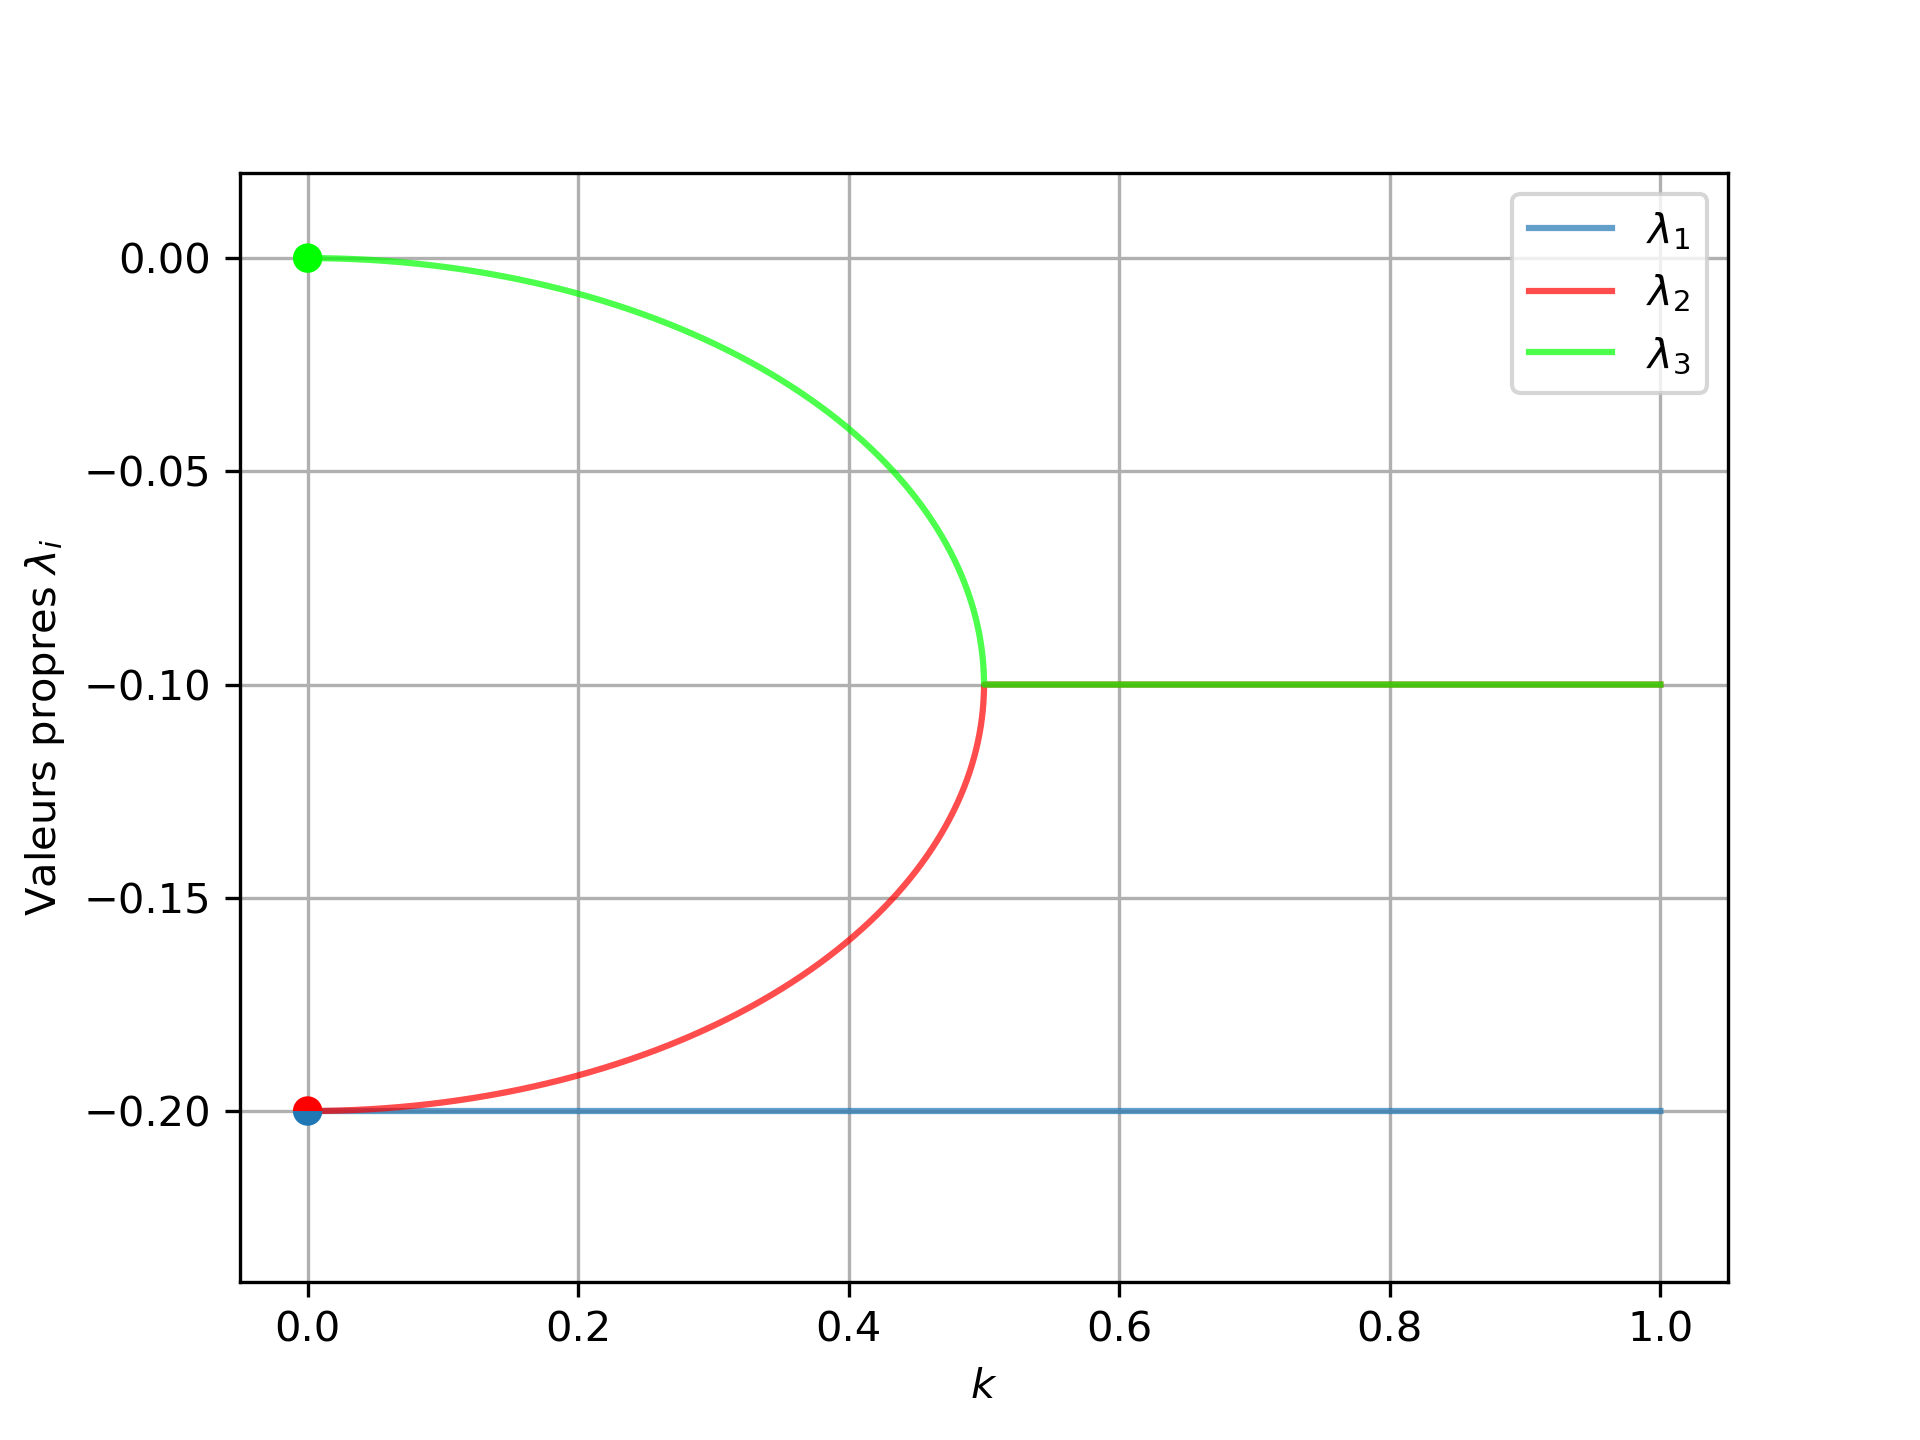
\includegraphics[width=\textwidth]{images/couplee/eigenvalues_eps=0.2.png}
         \caption{}
         \label{fig:eigenvals}
     \end{subfigure}
     \hfill
     \begin{subfigure}[b]{0.62\textwidth}
         \centering
         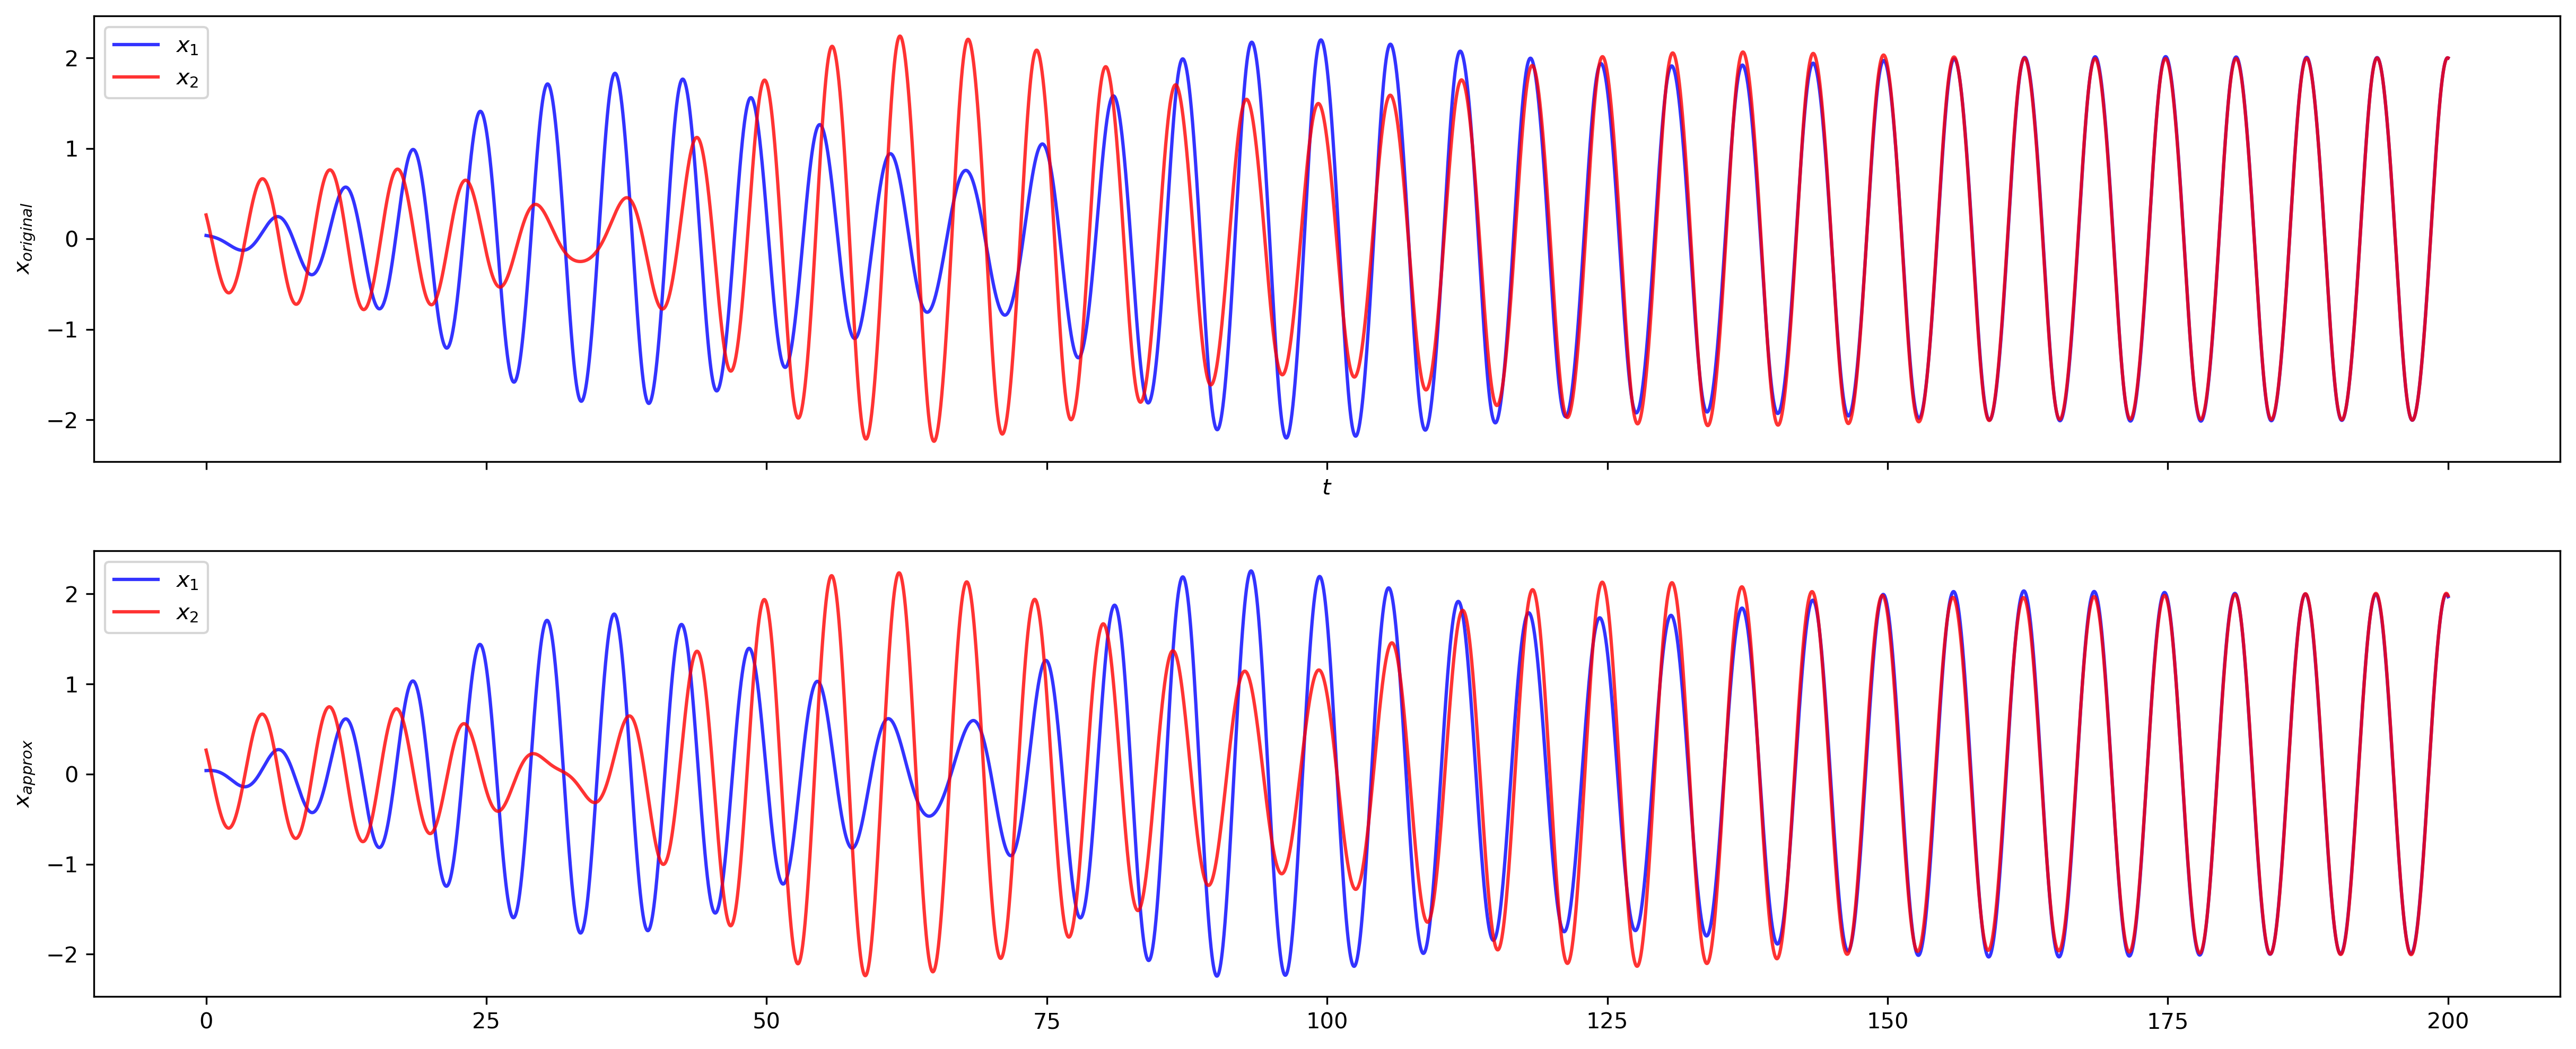
\includegraphics[width=\textwidth]{images/couplee/notitle_k=1_x0=[0.038,-0.018,0.265,-0.486]_eps=0.1.png}
         \caption{}
         \label{fig:comparison}
     \end{subfigure}    

    
    % \subcaptionbox{}[.37\linewidth]{%
    %     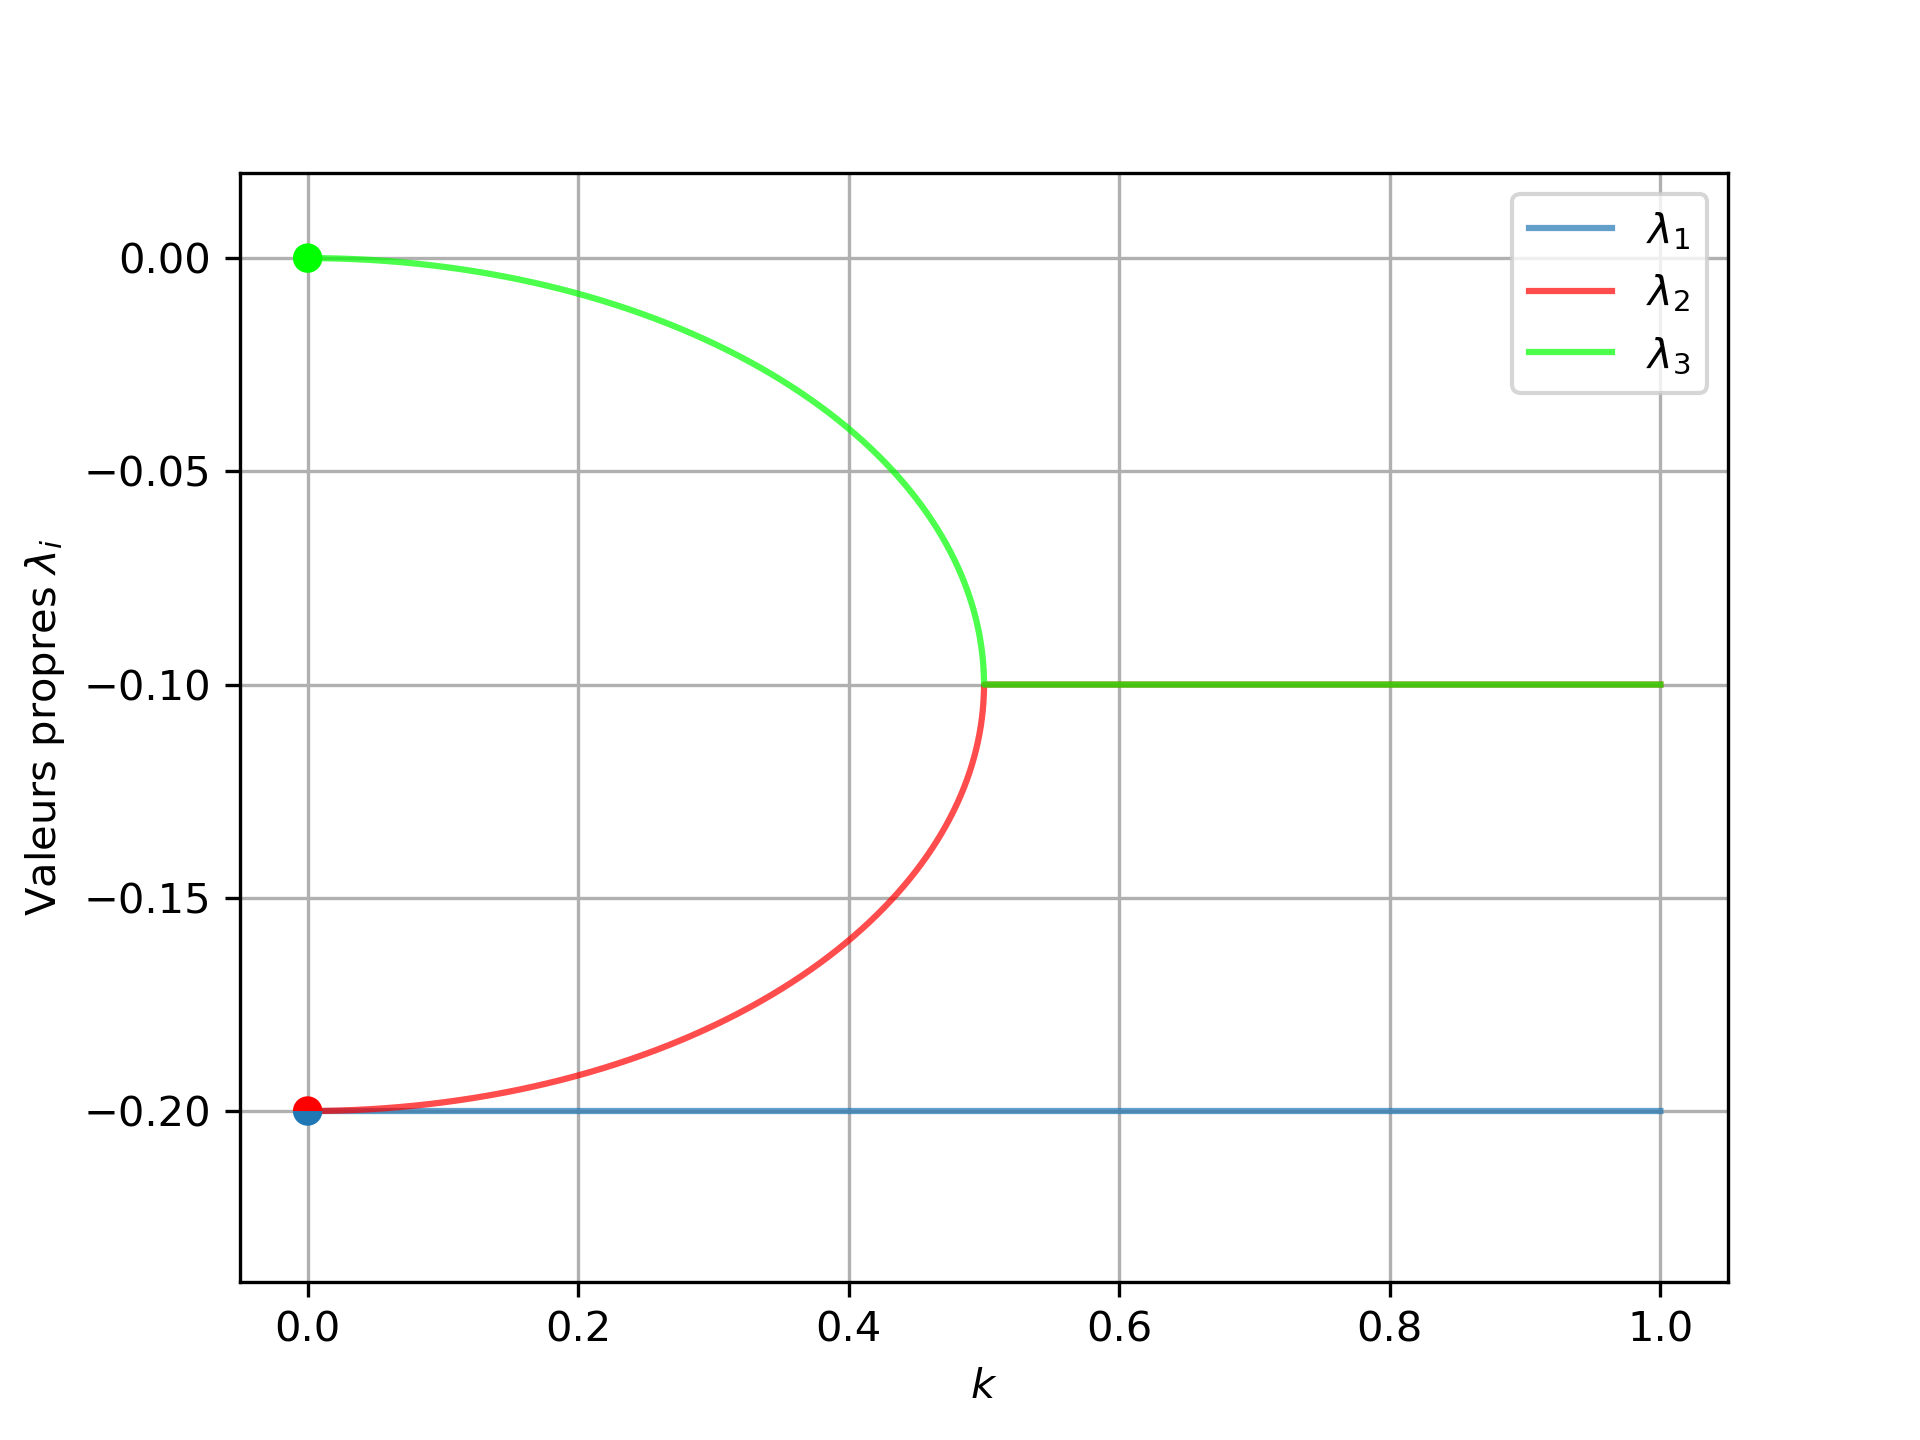
\includegraphics[width=\linewidth]{images/couplee/eigenvalues_eps=0.2.png}%
    %     \label{fig:eigenvals}
    % }
    % \hfill
    % \subcaptionbox{}[.60\linewidth]{%
    %     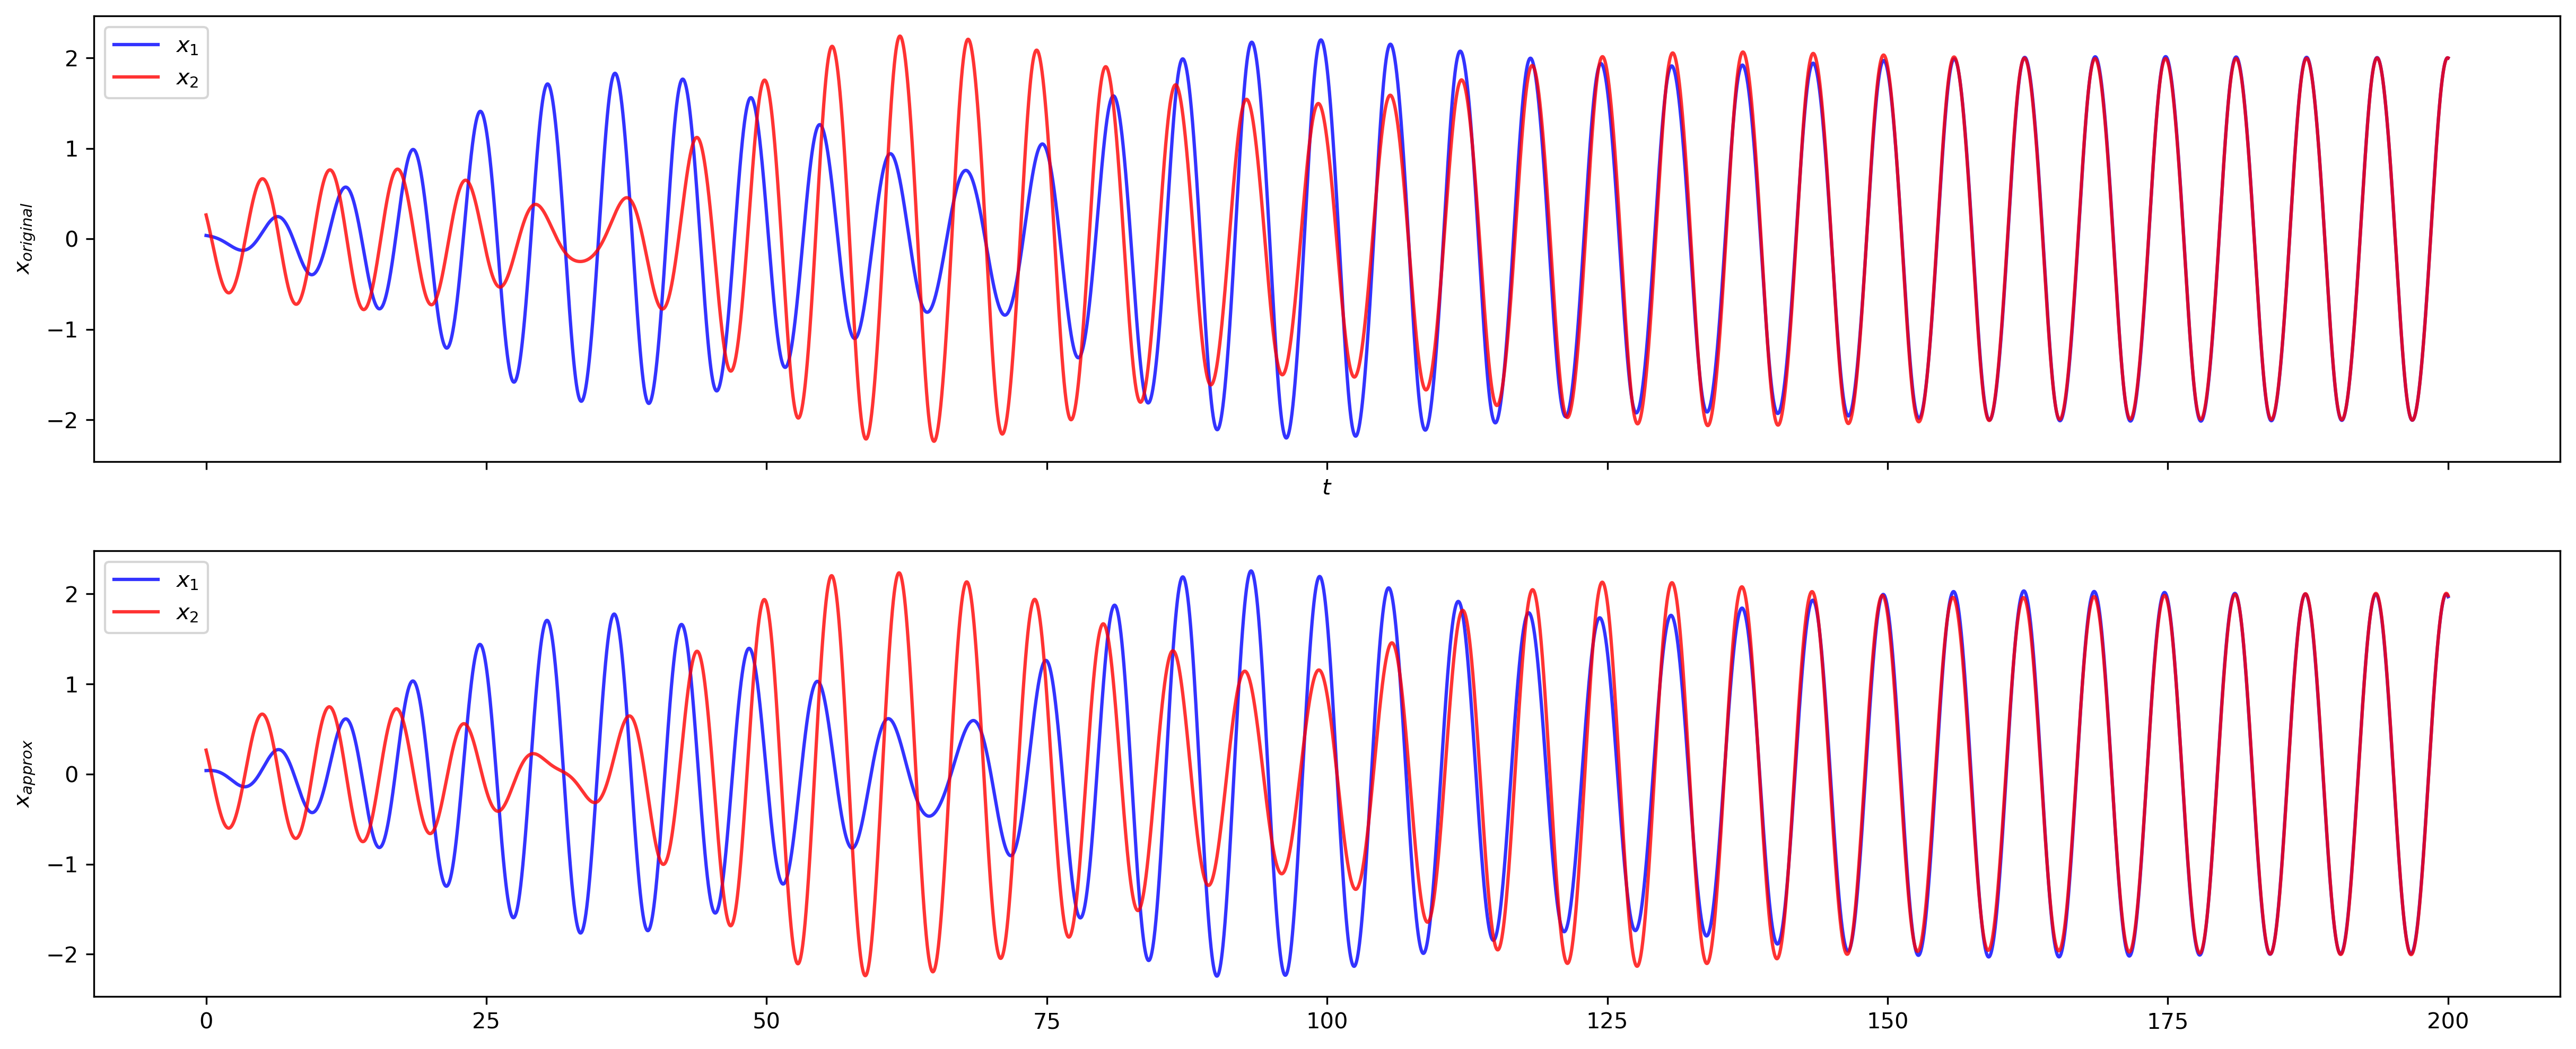
\includegraphics[width=\linewidth]{images/couplee/notitle_k=1_x0=[0.038,-0.018,0.265,-0.486]_eps=0.1.png}%
    %     \label{fig:comparison}
    % }

    \caption{\textbf{(a)} Tracé de la partie réelle des valeurs propres $\lambda_i$ en fonction de $k$, $\epsilon=0.2$. 
        \textbf{(b)} Comparaison graphique du système original \eqref{eq:coupled_vdp} avec le système moyenné \eqref{eq:slow_flow} faite par intégration numérique, notez les amplitudes oscillantes – $x_1(0)=0.038$, $x_2(0)=0.265$, $\dot{x}_1(0)=-0.018$, $\dot{x}_2(0)=-0.486$, $\epsilon=0.1$, $k=1$}
    
\end{figure}

%
Il est évident que $\lambda_1$ est strictement négatif. %$\lambda_1 < 0 \ \forall k$
Et pour $0 \leq |k| \leq \frac{1}{2} $ on voit que $\sqrt{\epsilon^2 - 4\epsilon^2k^2} \leq \epsilon$, donc :
\[ -\epsilon \leq \lambda_2 \leq -\frac{\epsilon}{2} \qquad -\frac{\epsilon}{2} \leq \lambda_3 \leq 0\]
%
Lorsque $|k| > \frac{1}{2}$, $\lambda_2$ et $\lambda_3$ deviennent un couple de complexes conjugués. 
Géométriquement, cela correspond à des trajectoires spirales oscillant autour du point stationnaire 
– effectivement, on peut vérifier numériquement que $r_1$, $r_2$ et $\Theta$ oscillent dans ces cas-là (fig. \ref{fig:comparison}). 
La stabilité est déterminée par la partie réelle des valeurs propres. Or :
\[ \Re(\lambda_2) = \Re(\lambda_3) = -\frac{\epsilon}{2} \]
%
La partie réelle des trois valeurs propres étant toujours négatives, 
on voit donc que dans le cadre de notre approximation, les points stationnaires $(2, 2, 0)$, $(2, 2, \pi)$ sont stables pour tout $k$. 
Ce qui nous montre que les deux oscillateurs peuvent se synchroniser soit en phase ou en anti-phase. 
On n'a pas éliminé la possibilité que l'oscillateur ne se synchronise pas, ni qu'il pourrait y avoir d'autres solutions stables. 
Pour cela, il faudrait étudier l’existence d’autres solutions stationnaires stables ou de conditions ‘neutres’ qui ne donnent pas lieu a la synchronisation.
%
Ceci dit, l’analyse numérique du problème 
%par intégration numérique 
avec conditions initiales aléatoires n’a pas révélé d’autre solution stables, ni de cas non synchronisant.
% Pour cela, il faudrait étudier de plus près l'étendu des bassins d'attraction - s'il y a des conditions 'neutres' 
% qui ne donnent pas lieu à de la synchronisation.

Étant donné que les valeurs propres des deux points stationnaires sont identiques, 
on s'attend a ce que les deux configurations synchronisées soient aussi stables l'une que l'autre. 
Donc a priori, si le système n'admet pas d'autres solutions stables, l'état synchronisé devra dépendre des conditions initiales.